\documentclass{matmex-diploma-custom}
\usepackage{amsfonts}
\usepackage{algorithm}
\usepackage{algpseudocode}

\makeatletter
\renewcommand{\ALG@name}{Алгоритм}
\makeatother

\begin{document}
\filltitle{ru}{
  chair = {Кафедра Системного Программирования},
  title = {Построение генетических карт по неполным и зашумленным данным},
  type = {diploma},
  position = {студентки},
  group = 545,
  author = {Крамар Алина Сергеевна},
  supervisorPosition = {к.\,ф.-м.\,н., доцент},
  supervisor = {Сысоев С.\,С.},
  reviewerPosition = {науч. сотрудник.},
  reviewer = {Добрынин П.В.},
  chairHeadPosition = {д.\,ф.-м.\,н., профессор},
  chairHead = {Терехов А.\,Н.},
  university = {Санкт-Петербургский Государственный Университет},
  faculty = {Математико-механический факультет},
  city = {Санкт-Петербург},
  year = {2014}
}
\filltitle{en}{
  chair = {Department of Software Engineering},
  title = {Genetic linkage mapping based on incomplete and noisy data},
  author = {Alina Kramar},
  supervisorPosition = {associate professor},
  supervisor = {Sergey Sysoev},
  reviewerPosition = {research associate},
  reviewer = {Pavel Dobrynin},
  chairHeadPosition = {professor},
  university = {Saint Petersburg State University},
  chairHead = {Andrey Terekhov}
}
\maketitle \tableofcontents
\section*{Введение}

Краткая медицинская энциклопедия \cite{petrovsky1989} даёт следующее
определение слову “генетика”: наука о наследственности и изменчивости
организма. Согласно законам наследования все основные признаки и
свойства любых организмов определяются и контролируются единицами
наследственной информации - генами, локализованными в специфических
структурах клетки - хромосомах
\cite{griffiths2005introduction,griffiths2000introduction}. В связи с
этим основной задачей генетики является на основе первичной структуры
биополимеров (молекул ДНК или РНК) определить фенотип особи, механизмы
наследования тех или иных признаков и т.п. Получение информации о
первичной структуре ДНК называется секвенированием \cite{cito1994}. К
сожалению, современные методы секвенирования не в состоянии
предоставить информацию о полной нуклеатидной последовательности в
рамках конкретной хромосомы \cite{molecular}. Сама по себе
нуклеатидная последовательность не содержит прямой информации о
происхождении того или иного однозначно идентифицируемого участка
(маркера), и поэтому довольно сложно определить, от какого предка был
унаследован тот или иной признак. Для определения шаблонов
наследования и выявления его принципов используются генетические карты
хромосом \cite{morgan1922mechanism}.

Генетическая карта - это схема или порядок расположения маркеров на
хромосоме (здесь и далее подразумевается структурный маркер,
т.е. маркер, имеющий отличимое нуклеатидное представление, которое
позволяет его идентифицировать) и генов. Зачастую, наличие генов не
так важно, как наличие маркеров, потому что гены имеют свойство
наследоваться не полностью \cite{schiller2010genome}. Идея создать
генные карты принадлежит Томасу Моргану, внёсшему огромный вклад в
теорию наследственности. Его идея была связана с явлением сцепленного
наследования генов. Из-за мейотического кроссинговера, который делает
невозможным полностью коррелированное наследование маркеров и влияет
на расхождение сцепленных генов по разным гаметам, у Моргана появилось
предположение о существовании связи между физическим расстоянием между
маркерами и их взаимодействием в процессе наследования
\cite{creighton1931correlation}. Это предположение подтвердилось в
1913 году учеником Моргана Альфредом Стёртевантом, построившим первую
генетическую карту на основе данных Drosophila melanogaster
\cite{goldhor1962genetics,sturtevant1939introduction}.

Кроссинговер на этапе мейоза вносит возмущение в сцепленное
наследование \cite{creighton1931correlation}, и чем чаще он
проявляется, тем чаще наблюдается отклонение от сцеплений. Физическое
расстояние между парой генов прямо пропорционально вероятности
кроссинговера, что позволяет однозначно расположить маркеры на
молекуле \cite{sturtevant1939introduction}. Генетическое расстояние не
трудно перевести в физическое, но чаще всего в этом нет необходимости,
так как генетическая карта несёт структурный характер и для механизма
наследования существенен порядок \cite{hartl2011genetics,
  malacinski2005essentials} исследуемых маркеров. Единицей измерения
расстояния является 1 сантиморган (1 cM). Стоит упомянуть, что задача
построения генетической карты хромосомы имеет смысл для диплоидных
особей и лучше решается, когда исследуемые особи находятся в родстве
\cite{meiosi}. Задача так же решается проще с помощью данных о
семействах особей, которые размножаются c большой скоростью (Быстрое
размножение и большое количество потомков позволяют секвенировать
большее количество особей из разных поколений за меньший период,
поэтому данные о таких родословных получаются наиболее
информативными), поэтому большее количество карт на данный момент
имеют хромосомы дрозофил, кошек, мелких грызунов и насекомых
\cite{mcpeek1996introduction}. В данном исследовании нас интересуют
генетические карты человека, так как эти карты являются единственным
способом проведения генетического анализа на наличие и
предрасположенность особи к тяжёлым наследственным заболеваниям. С
помощью генетического анализа можно выявлять болезнь Альцгеймера
\cite{schellenberg1992genetic}, гемофилию \cite{oberle1985genetic},
хорею Хаттингтона \cite{anderson2004polymorphic} и т.п.

Современные средства генетического картирования позволяют построить
карту по файлу с данными о родословной в определённом формате
\cite{lander1987mapmaker, crimap, faslinkUrl}. Причём не обязательно
иметь полную информацию о степени родства, половой принадлежности и
возрасте рассматриваемых особей. Более того, результаты секвенирования
могут содержать ошибки.

Общепризнанными \cite{kruglyak1996parametric} и наиболее
распространёнными методами генетического картирования являются:
\begin{itemize}
\item Алгоритм Элстона-Стюарта
\item Алгоритм Ландера-Грина
\end{itemize}

Программные средства, основанные на вышеуказанных алгоритмах, хорошо
решают поставленную задачу на взятом у человеческих особей материале
при сравнительно небольшом (по сравнению с количеством известных науке
видами маркеров) количестве маркеров [Алгоритм Элстона---Стюарта] и
исследуемой семьи для небольшого размера [Алгоритм
Ландера---Грина]. Практические требования современной медицины
приводят к необходимости строить генетические карты по все большим и
большим наборам маркеров. Вычислительная сложность алгоритма
Элстона-Стюарта зависит от количества исследуемых маркеров
экспоненциально \cite{fishelson2002exact}, поэтому время рыботы
алгоритма растёт с увеличением данного параметра. В результате чего
генетическое картирование этим методом становится неосуществимым на
практике. Алгоритм Ландера-Грина позволяет исследовать большее
количество маркеров, но на данных о семействах меньшего размера, так
как время работы этого алгоритма экспоненциально растёт с увеличением
количества наблюдаемых в родословной особей-``непрародителей''
(особей, родители которых присутствуют в исследуемом множестве особей)
\cite{fishelson2002exact}.

В 2013 году в работе \cite{sysoev} Сергеем Сысоевым был предложен
алгоритм построения генетической карты путём прямого извлечения
информации о генетических расстояниях между маркерами без учёта
кратности кроссинговера. Вычислительная сложность данного алгоритма
имеет полиномиальную зависимость зависит как от количества маркеров,
так и от мощности множества особей в рассматриваемой родословной, что
делает данный алгоритм перспективнее ранее упомянутых для решения
задач современной генетики. При этом алгоритм прямого извлечения
данных имеет ряд существенных недостатков, а именно:
\begin{enumerate}
\item Плохая теоретическая обоснованность.

  В работе \cite{sysoev} Сысоевым утверждается, что алгоритм извлекает
  всю возможную информацию о рекомбинациях маркеров в исследуемых
  особях. В главе \textbf{1.3} мы покажем, что это утверждение вообще
  говоря неверно.

\item Отсутствие верификации.

  Алгоритм был проверен только на небольшой семье кошек из 192 особей
  и рассматривал 35 маркеров. На других данных алгоритм не проверялся.

\item Неверный результат в случае кратности кроссинговера.

  Это существенно снижает полезность алгоритма, так как в природе
  неоднократный кроссинговер --- явление, встречающееся достаточно
  часто.

\end{enumerate}

Исходя из этого, цель данной работы можно сформулировать следующим
образом: предложить новый алгоритм построения генетических карт на
основе предложенного в статье \cite{sysoev} метода, усовершенствовав
алгоритм в части учёта кратных рекомбинаций, верифицируя полученный
алгоритм на реальных и синтетических данных, сравнив результаты работы
нового алгоритма с результатами и характеристиками работы аналогов.

\section{Обзор существующих решений}

\subsection*{Основные понятия}

Для того, чтобы рассматривать существующие подходы, нужно более
формально поставить задачу, которую они решают. Нам потребуются
следующие понятия \cite{dictionary}:
\begin{description}
\item[Маркер(ДНК-маркер)] --- полиморфный признак, выявляемый на
  уровне нуклеотидной последовательности ДНК.
\item[Локус] --- положение маркера на генетической или цитологической
  карте.
\item[Аллель] --- вариант последовательности ДНК в текущем локусе.
\item[Гомозигота] --- диплоидная (двойной набор одинаковых хромосом)
  особь, копия генов которой представлена одинаковыми аллелями.
\item[Гетерозигота] --- диплоидная особь, копия генов которой
  представлена разными аллелями.
\end{description}

Поясним введённые выше понятия примером. Информацию об особи будем
записывать в виде строки вида \textbf{AaBb}, где \textbf{A} --- вид
маркера в отцовской хромосоме в позиции 1, \textbf{a} --- вид маркера
в материнской хромосоме в позиции 1, \textbf{B} --- вид маркера в
отцовской хромосоме в позиции 2, \textbf{b} --- вид маркера в
материнской хромосоме в позиции 2. В данном примере особь
гетерозиготна в позициях 1 и 2, так как имеет разные маркеры от отца и
матери. Если бы в позиции 2 находилась строка \textbf{BB}, то особь
была бы гомозиготна, так как маркеры одинаковые.

\begin{description}
\item[Гамета] --- одинарный набор хромосом. В нашем случае,
  подстрока последовательности аллелей, содержащая половину
  генетического материала.

\item[Фаза] --- различают две фазы: CIS и TRANS. CIS --- расположение
  доминантных генов на одной хромосоме, а TRANS --- расположение
  доминантных генов на разных хромосомах. Фаза имеет смысл только для
  особей, гетерозиготных в обоих локусах.
\end{description}

В нашем примере особь \textbf{AaBb} находится в фазе CIS, так как
доминантные признаки (символы в верхнем регистре) находятся на одной
хромосоме. \textbf{AabB} --- пример TRANS фазы.

\begin{description}
\item[Рекомбинация] --- перераспределение генетического материала
  родителей в потомстве.
\end{description}

В приведённом выше примере при образовании особью гаметы, которая
передастся потомкам, могут возникнуть следующие сочетания:
\textbf{AB}, \textbf{Ab}, \textbf{aB} и \textbf{ab}. Получить
информацию о наличии рекомбинации мы можем, зная фазу. Для CIS-фазы (в
нашем случае, особь представляется строкой \textbf{AaBb} или
\textbf{aAbB}), рекомбинантными будут являться гаметы \textbf{aB} и
\textbf{Ab}, в случае же TRANS-фазы (особь --- строка вида
\textbf{AabB} или \textbf{aABb}), рекомбинантными являются гаметы
\textbf{ab} и \textbf{AB}.

\begin{description}
\item[Генетическая карта] --- схема расположения маркеров на
  хромосоме.
\item[Кроссинговер(Перекрёст)] --- процесс обмена участками
  гомологичных хромосом.
\end{description}

Перейдём к алгоритмическому смыслу задачи и рассмотрим пути её
решения. Имея на входе данные о родословной, количестве исследуемых
маркеров, о нуклеотидных последовательностях всех особей, а так же о
их родственной связи, генетическую карту можно построить с помощью
следующих алгоритмов, имеющими программную реализацию
\cite{fishelson2002exact}:
\begin{itemize}
\item Алгоритм Элстона - Стюарта
\item Алгоритм Ландера - Грина
\item Построение генетических карт по полностью секвенированным
  участкам геномов (Сысоев)
\end{itemize}

Алгоритм Элстона-Стюарта, так же как и алгоритм Ландера-Грина, трудно
назвать алгоритмами в классическом понимании этого слова, так как они
не предоставляют собой рабочего механизма, приводящего сразу к ответу,
а скорее позволяют привести задачу в биологической и формальной
формулировке в задачу в математической записи, которая хорошо изучена,
имеет решения и хорошо моделируется. Так, например, алгоритм
Ландера-Грина формулирует задачу генетического картирования в терминах
скрытых марковских цепей, а алгоритм Элстона-Стюарта оптимизирует
функционал правдоподобия для конкретной родословной, упрощая его
вычисления.

\subsection{Алгоритм Элстона-Стюарта}

Нам известно, что генотип родителя влияет на генотип ребёнка, поэтому
можем записать вероятность генотипа потомка как $$P(G_{founder}).$$
Также мы знаем, что вероятность генотипа потомка контролируется
родительскими генотипами $$P(G_{offspring} | G_{mother},
G_{father}).$$ Алгоритм Элстона-Стюарта, как и алгоритм Ландера-Грина,
не связывает частоту рекомбинаций с расстоянием между генами и не
рассматривает влияние расстояния на сцепление при наследовании, что в
нашем случае означает, что вышеуказанная изначально никак не
параметризуется.

Вероятность наблюдаемого фенотипа контролируется генотипом $$P(X_{i} |
G_{i}).$$ Рассмотрим функционал правдоподобия для задачи генетического
картирования в общем случае, используя записанные выше вероятности
\cite{elston1971general}: $$L =
\Sigma_{G_{1}}...\Sigma_{G_{n}}Pi_{\{o,f,m\}}P(G_{o} | G_{f}, G_{m})
Pi_{i}P(X_{i} | G_{i})$$.

Если обратить внимание на запись вероятностей родительского генотипа,
потомка данного родителя и вероятность фенотипа данного ребёнка, в
попробовать посчитать их в случае родословных без кровосмесительных
``браков'' и содержащих не более чем два поколения (иначе говоря,
каждая особь из родословной является либо родителем, либо ребёнком),
то можно заметить, что большинство вероятностей оборачивается в ноль
(так как нет зависимости).

Используя это наблюдение, можно записать новый функционал
правдоподобия, актуальный для семейств из двух поколений.$$L =
\Sigma_{G_{founder}}P(X_{founder}|G_{founder})H(G_{founder})P(G_{founder})$$
--- где $H_{j}(G_{i})$ --- вероятность наличия у $G_{j}$ детей вместе
с $G_{i}$. При максимизации данного функционала, просмотр особей
начинается с нижнего уровня, из-за превращения в ноль большой части
вероятностей.

Нетрудно увидеть, что максимизация описанного функционала
правдоподобия имеет большую вычислительную сложность, а именно
экспоненциальный рост времени выполнения с увеличением количества
исследуемых маркеров \cite{fishelson2002exact}. Плюсами данного
алгоритма является хорошая применимость в случае потенциально больших
семейств, или в случае конечного и малого количества исследуемых
маркеров.

Данный алгоритм имеет не единственную программную реализацию, но для
сравнения алгоритмов в конце данной работы мы будет использовать пакет
FASTLINK \cite{faslinkUrl}, так как это самая последняя версия
алгоритма, а значит, и наиболее надёжная.

\subsection{Алгоритм Ландера-Грина}

В отличии от алгоритма Элстона-Стюарта, алгоритм Ландера-Грина основан
на другом предположении о вероятных рекомбинациях
\cite{lander1987construction}: связь вероятности рекомбинации в
позиции $n$ с вероятностью рекомбинации в позиции $n-1$. По данной
модели не трудно построить скрытую марковскую цепь. Если не вдаваться
в подробности, то мы, чтобы получить данные о той или иной позиции
должны рассмотреть все предшествующие и последующие маркеры.

Запишем вероятные фенотипы в виде $X_{i}$, а состояние идентичных по
происхождению аллелей в каждом локусе $I_{i}$, где $i \in
(1:M)$. Запишем вероятность проявляемого фенотипа в зависимости от
состояния генотипа как $$P( X_{i} | I_{i}).$$ Воспользуемся
предположением, что вероятность рекомбинации в позиции $n$ обусловлена
вероятностью рекомбинации в позиции $n-1$. Запишем эту вероятность
как $$P(I_{i-1}|I_{i}).$$ Используя описанные вероятности получаем
функционал правдоподобия, записанный следующим образом: $$L =
\Sigma_{I_{i}}...\Sigma_{I_{M}}P(I_{i})\Pi_{i=2}^{M}P(I_{i}|I_{i-1})\Pi^{M}_{i=1}P(X_{i}|I_{i}).$$
Схема скрытой марковской цепи при этом выглядит изображённым на
Рис. образом.

Нетрудно заметить, что максимизировать данный функционал достаточно
трудоёмко. У этого подхода экспоненциальная вычислительная сложность,
зависящая от объёма родословной \cite{lander,
  fishelson2002exact}. Т.о. при исследовании больших семейств этот
алгоритм неэффективен и может не завершиться. Зато он позволяет
исследовать любое число маркеров, что делает его более удобным для
решения задач современной генетики, так как исследуемые геномы
становятся сложнее по структурному (маркерному) представлению, а
исследуемые родословные не настолько большие по количеству особей. Так
же данный алгоритм позволяет исследовать семьи с кровосмесительным
спариванием, например, семьи кошек, мелких грызунов и т.п.

Данный алгоритм так же имеет реализованное программное средство CRIMAP
\cite{crimap}, которое будет принимать участие в сравнении алгоритмов
генетического картирования, проводимом в рамках данной работы.

\subsection{Построение генетических карт по полностью секвенированным
 участкам геномов (genmap)}

Предыдущие алгоритмы были основаны на предположении, что процесс
передачи генов --- это лишь вероятностный процесс, и не учитывали
специфику образования гамет и передачи наследственной
информации. Использовать в качестве данных о происхождении аллели
данные из прямых потомков и предков на основе результатов их
секвенирования было предложено С. Сысоевым в 2013 году. Его алгоритм
был основан на знании о том, что частота рекомбинаций между двумя
маркерами прямо пропорциональна расстоянию между ними \cite{sysoev}. В
генетическом картировании появилась новая идея не максимизировать
функционал правдоподобия, а смотреть на структурное представление ДНК
конкретной особи и извлекать информацию из него. Также в статье
\cite{sysoev} продемонстрирована лучшая вычислительная сложность,
которая является полиномиальной, а так же хорошая точность в случае с
реальными данными кошек, которые, как известно, не укладываются в
область применения алгоритма Элстона-Стюарта.

Недостатком данного алгоритма является его неопробованность, зато к
уверенным достоинствам можно отнести полиномиальную сложность и
удобство использования. Данный алгоритм имеет программное средство в
виде скрипта на языке Python2 и будет использовано нами в качестве
базы для собственной реализации.

\subsection*{Построение генетических карт}

Поскольку существующие алгоритмы имеют большую вычислительную
сложность или не способны давать правильный ответ в наиболее частых случаях,
было решено написать новый алгоритм, позволяющий строить генетические
карты быстрее и качественнее, чем у существующих. Так как в случае с
экспоненциальным ростом (алгоритм Элстона-Стюарта и алгоритм
Ландера-Грина) помочь могут только локальные оптимизации
\cite{o2001rapid, fishelson2002exact, fishelson2004optimizing}, не влияющие на
асимптотическую скорость, разумно предположить, что развивать стоит
алгоритм прямого извлечения данных о рекомбинациях из полностью
секвенированных геномов, рассмотренный в главе \textbf{1.3}.

\section{Постановка задачи}

Обзор существующих решений показал, что ни один из существующих
алгоритмов генетического картирования не является полноценным и
удобным способом решения решения возникающих в современной генетике
задач. Тем не менее недостатки алгоритма, предложенного в \textbf{1.3}
могут быть устранены или сведены к минимуму.

Таким образом, целью данной работы является написание нового алгоритма
генетического картирования на базе метода прямого извлечения данных.

\bigskip

Для достижения поставленной цели был сформулирован ряд задач:

\begin{enumerate}
\item Доработка алгоритма прямого извлечения данных
\item Верификация полученного алгоритма
  \begin{enumerate}
  \item моделирование и генерация тестовых
    данных
  \item сравнение существующих алгоритмов с полученной версией
  \end{enumerate}
\end{enumerate}

\section{Доработка алгоритма}

\subsection{Анализ недостатков и их исправления}

\subsubsection{Восстановление расположения маркеров по матрице
  попарных расстояний}

В статье Сысоева \cite{sysoev} утверждается, что алгоритм использует
всю информацию о происхождении аллели, которую возможно получить из
предоставляемых данных. Для более точного представления процесса
работы алгоритма была нами сформулирована его основная мысль: алгоритм
упорядочивает набор маркеров на хромосоме, используя для этого матрицу
попарных расстояний. Вообще говоря, непосредственно матрицу попарных
расстояний на этапе построения мы получить не можем
\cite{bohonak2002ibd}, поэтому алгоритм использует оценку матрицы,
основанную на частоте рекомбинаций. Как было сказано ранее, частота
рекомбинаций между двумя маркерами прямо-пропорциональна расстоянию
между ними \cite{stam1993construction}, поэтому матрицу попарных
расстояний мы оцениваем матрицей частот рекомбинации.

Так как реализация алгоритма не учитывает кратный кроссинговер, можно
предположить, что оценка матрицы попарных расстояний наиболее точна в
случае, если маркеры расположены друг к другу близко на хромосоме, так
как вероятность кроссинговера на отрезке малой длины меньше
вероятности кроссинговера на отрезке большей длины. На
Рис. \ref{fig:fig1} показан граф взаимных расстояний с
вершинами. Здесь видно, что по полученным данным можно представить
последовательность маркеров в виде точек, лежащих на одной прямой
(выстроить в линию).
\begin{figure}[h]
 \centering
  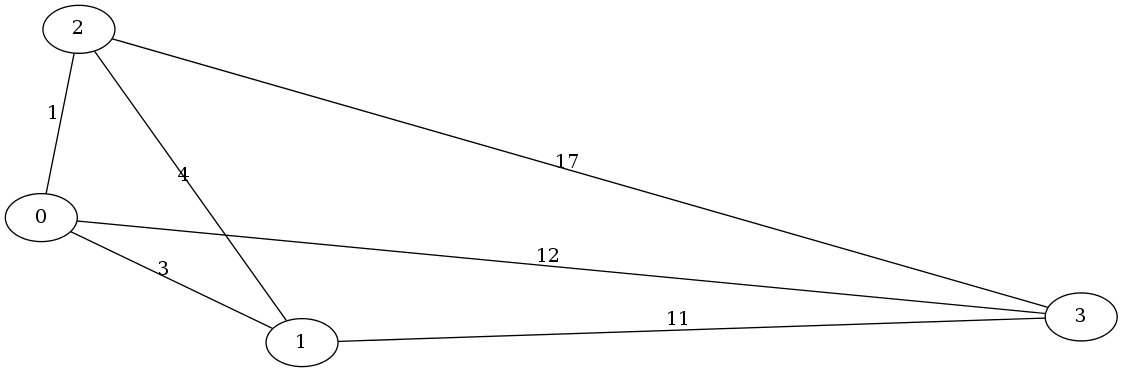
\includegraphics[width=1.0\textwidth]{good.png}
  \caption[width=0.4\textwidth]{Попарные расстояния в случае слабо
    удалённых маркеров}
  \label{fig:fig1}
\end{figure}

На Рис. \ref{fig:fig2} показана идентичная ситуация для выборки из
четырёх маркеров, далеко расположенных друг от друга.

\begin{figure}[h]
 \centering
  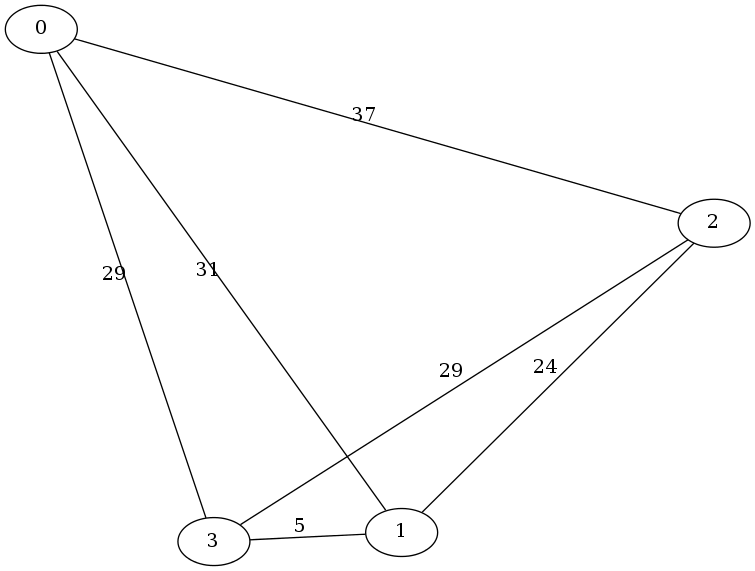
\includegraphics[width=0.7\textwidth]{bad.png}
  \caption[width=0.4\textwidth]{Попарные расстояния в случае сильно
    удалённых маркеров}
  \label{fig:fig2}
\end{figure}

Таким образом мы показали, что матрица частот рекомбинации является
оценкой матрицы попарных расстояний, причём оценка наиболее точна в
точках, находящихся близко друг к другу.

Согласно приведённым выше фактам, мы считаем, что наиболее правдивыми
данными в матрице являются пары маркеров с минимальной частотой
рекомбинаций между ними. Поэтому представляется уместным начать
строить карту от центра, определённого двумя самыми близкими
маркерами. Более формально этот алгоритм можно записать так, как
показано в листинге Алгоритм \ref{algo:linmark}.
\begin{algorithm}
  \caption{Лианеризация маркеров}
  \label{algo:linmark}
  \begin{algorithmic}[1]
    \Function{Linmark}{}

    \State $n \gets dim(distMatrix)$
    \State $(l, r) \gets \arg\!\min_{x, y} \mathit{distMatrix}[x][y]$
    \State $order \gets [l, r]$

    \While{есть не рассмотренные узлы}
    \State $l \gets first(order)$
    \State $r \gets last(order)$
    \State $m \gets $ ближайший к $l$ или $r$ узел.

    \If{$m$ ближе к $r$}
    \State $order \gets order + [m]$
    \Else
    \State $order \gets [m] + order$
    \EndIf
    \EndWhile
    \State \Return order
    \EndFunction
  \end{algorithmic}
\end{algorithm}

--- где входным параметром $distMatrix$ является квадратная матрица
частот рекомбинаций.

Применяя данный алгоритм, получаем результат в виде порядка маркеров.
На Рис. \ref{fig:fig3} видно (хоть представление и не линейно), что
есть некоторые ошибки, а так же видно, что эти ошибки порядка
допустимых транспозиций. В виде закрашенные узлов представлены
маркеры, порядковый номер которых не совпадает с порядковым номером в
полученном результате, т.е. ошибки.
\begin{figure}[h]
 \centering
  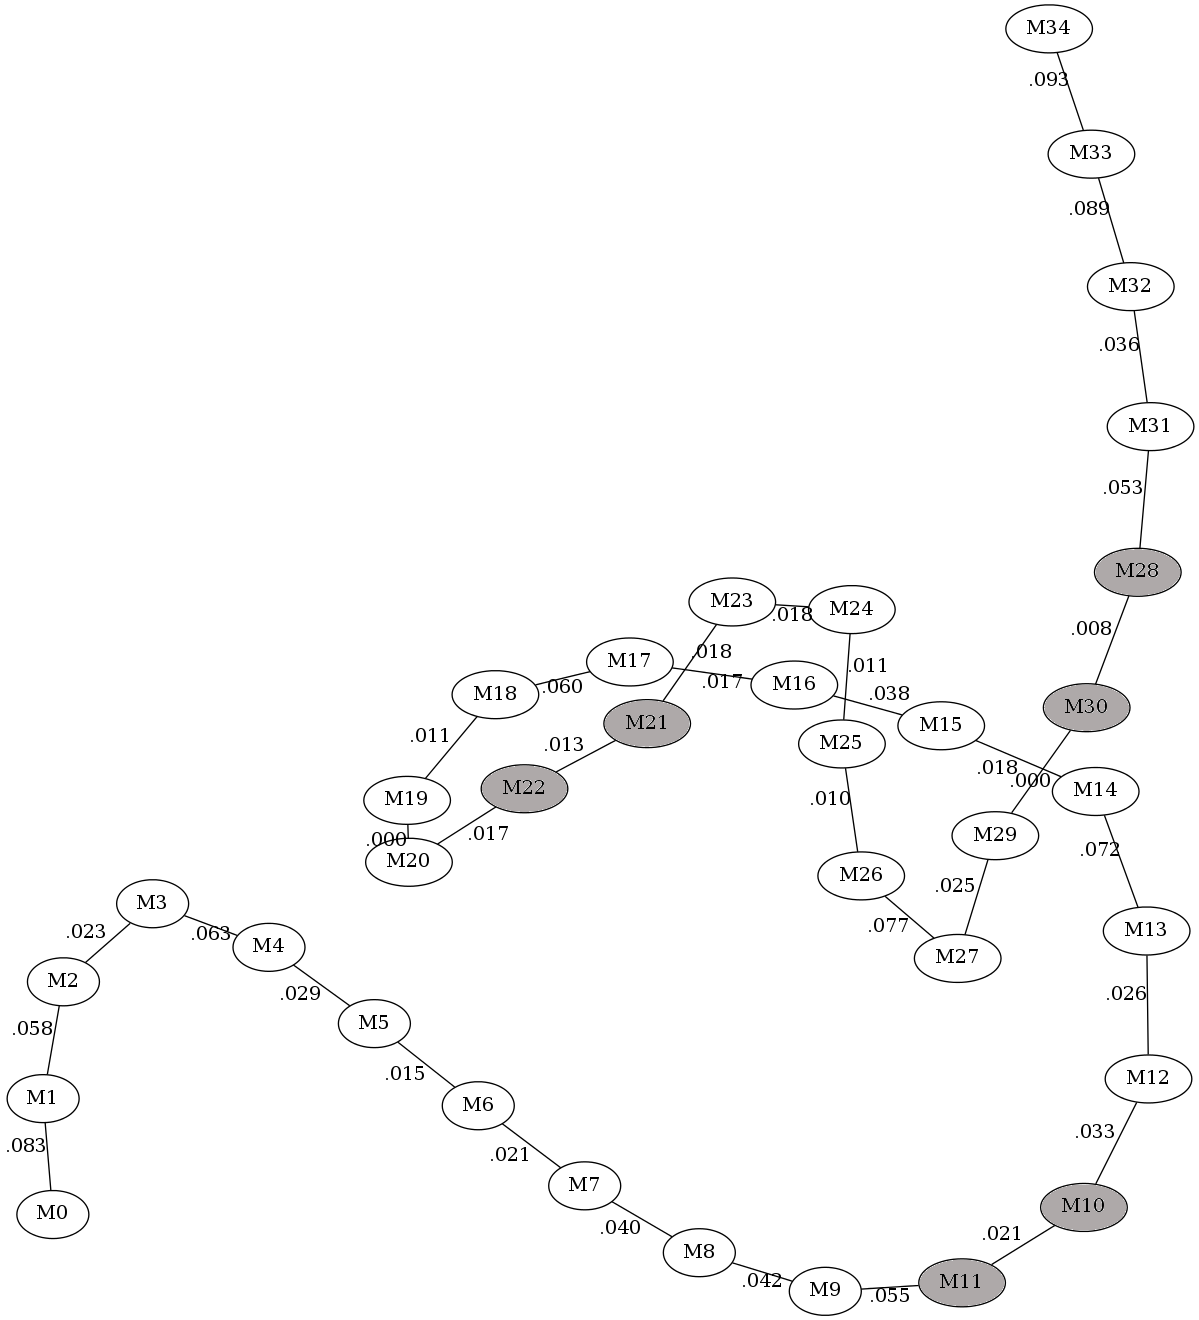
\includegraphics[width=0.85\textwidth]{linear.png}
  \caption[width=0.4\textwidth]{Порядок маркеров после применения
    алгоритма вытягивания в линию на семействе из 192 кошек с 35 маркерами}
  \label{fig:fig3}
\end{figure}
Посмотрев на рисунок можно попробовать представить изначальную матрицу
расстояний в виде графа с вершинами в маркерах и рёбрами с весами,
равными частоте рекомбинаций между двумя вершинами (в нашем случае ---
маркерами). Если вспомнить алгоритм построения минимального остовного
дерева Прима \cite{cormen2001introduction}, который основывается на
выборе ребра с минимальным весом, что в нашем случае эквивалентно
выбору пары маркеров с минимальным расстоянием между ними среди всех
остальных пар, то кажется логичным попробовать найти порядок маркеров
с помощью алгоритма Прима. Заметим так же, что можно получить искомый
порядок, введя нумерацию вершин минимального остовного дерева
(полученного с помощью алгоритма Прима) из графа попарных
расстояний. Результат будет точнее в случае наиболее точного
приближения матрицы попарных расстояний матрицей рекомбинаций.
\begin{figure}[h]
  \centering
  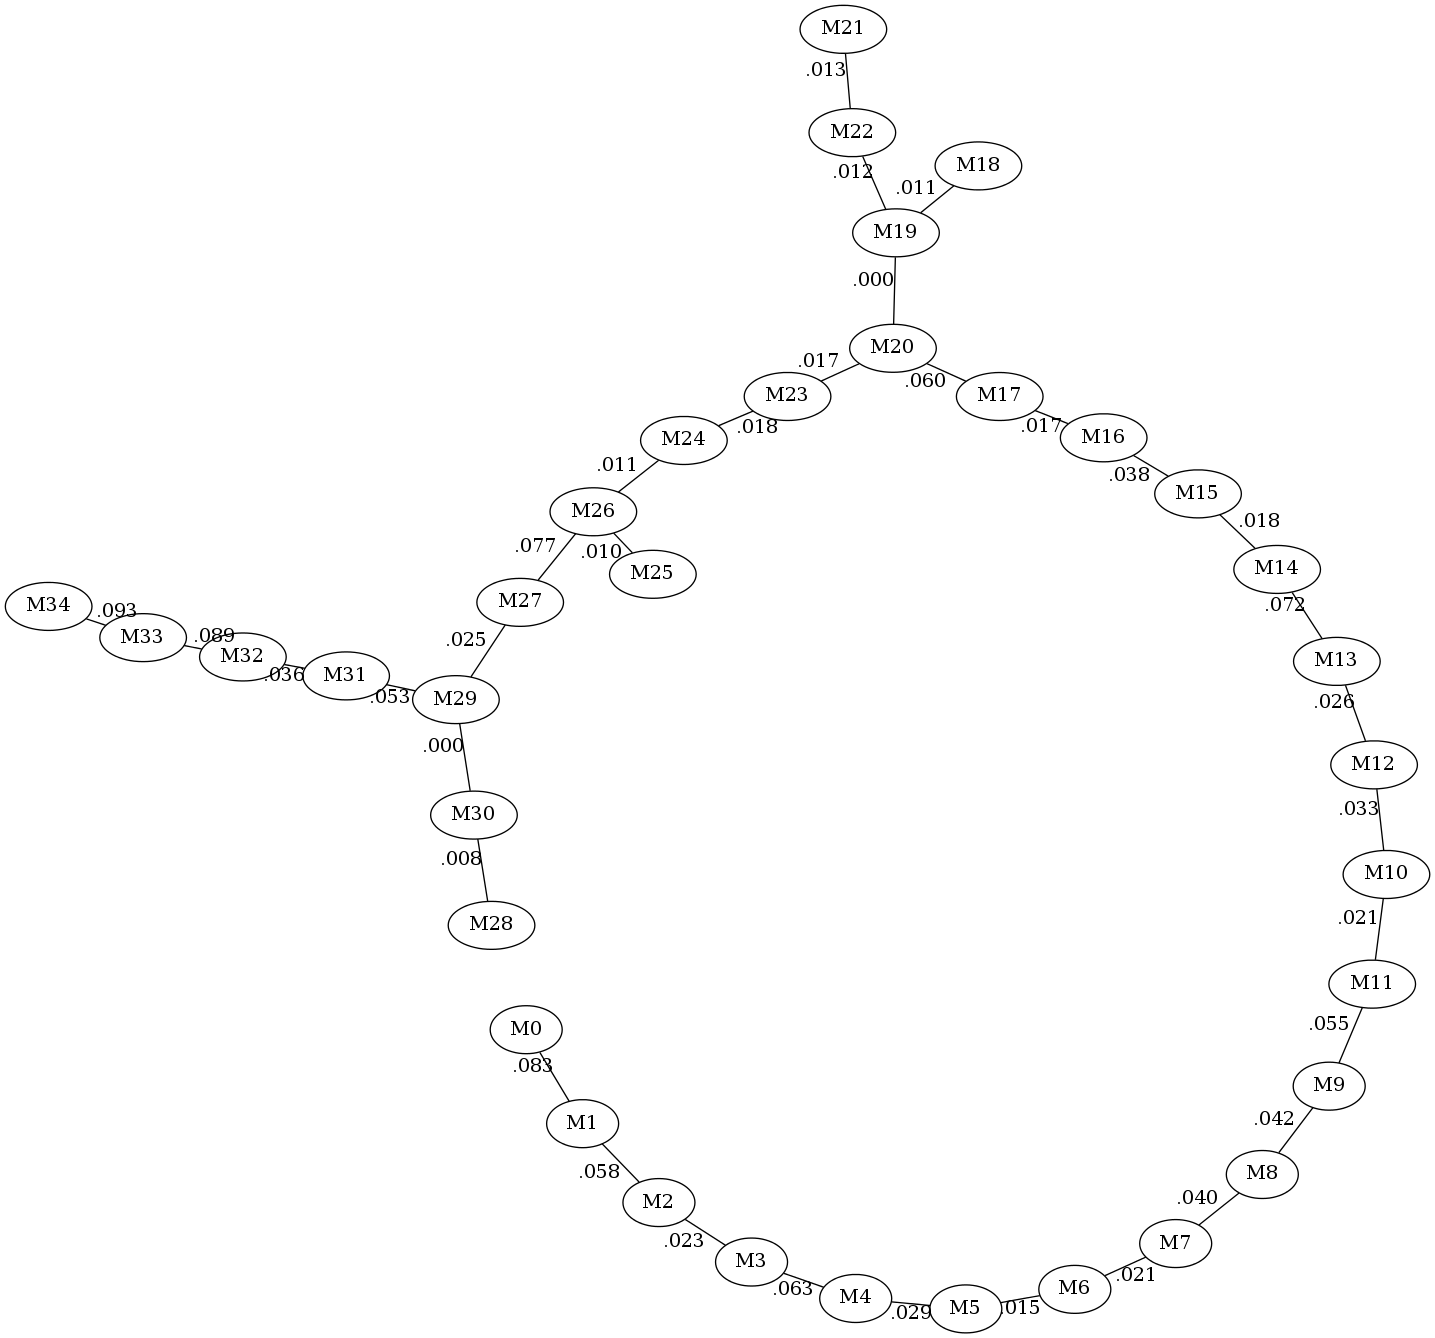
\includegraphics[width=0.85\textwidth]{prm.png}
  \caption[width=0.4\textwidth]{Минимальное остовное дерево графа
    попарных расстояний}
  \label{fig:fig4}
\end{figure}
На Рис. \ref{fig:fig4} представлено построенное с помощью алгоритма
Прима минимальное остовное дерево. Не трудно заметить, что те участки,
которые не имели нарушения порядка в первом варианте
[Рис. \ref{fig:fig3}] остались неизменными. Но там появились некоторые
особенности, из-за которых полученный граф не может называться линией
и упорядочить вершины (Аналогично Рис. \ref{fig:fig3} закрашены те
маркеры, порядок которых был определен неверно) простым способом. Эти
особенности вызваны либо наличием пар маркеров, между которыми не
наблюдалось рекомбинаций (.000 на графе), либо наличием пар маркеров,
лежащих друг от друга на большом расстоянии.

Данный пример показывает, что в задачах такого рода применимы основы
теории графов и правомерны предположения о наибольшем правдоподобии
маленьких расстояний. Кроме того, показанный алгоритм при правильной
организации хранения графа имеет вычислительную сложность
$O(M^2*log(M))$, что вносит небольшое улучшение в алгоритм, так как в
изначальной версии алгоритма сложность этапа построения порядка
маркеров составляла $O(M^3)$. Воспользоваться алгоритмом Прима мы
сможем в случае, если матрица частот рекомбинаций наиболее точно
приближает матрицу попарных расстояний.

\subsubsection{Повышение точности матрицы частот рекомбинаций}

Рассмотренные выше локальные оптимизации базируются на том, что
матрица попарных расстояний, полученная в результате извлечения
информации о происхождении аллели, правдоподобна. Мы уже показывали,
что для далеко отстающих друг от друга маркеров оценка не верна.

Не трудно заметить, что точность получаемого результата зависит от
точности матрицы частот рекомбинаций, так как в нашем случае именно
эта матрица является приближением матрицы попарных расстояний.  Как
было неоднократно замечено выше, алгоритм, на базе которого мы
пытаемся получить новое решение, не учитывает кратность кроссинговера,
в связи с чем матрица частот рекомбинации актуальна только в случае
однократного кроссинговера. Разумной является задача извлечения данных
о кратных рекомбинациях, так как это явление случается в природе
достаточно часто.

Попробуем рассмотреть функцию от расстояния между маркерами
$f(d):\mathbb{R} \to \mathbb{N}$, возвращающую количество произошедших
рекомбинаций. Очевидно, что эта функция неубывающая, потому что если
рекомбинация произошла на участке $[a, b]$, разделяющем два маркера,
то на более большом участке $[A, B] \supset [a, b]$ рекомбинаций
возможно не меньше, чем уже произошли. Однако первоначально нам не
известен порядок маркеров и расстояния между парой маркеров.

Заметим, что частичные сведения о порядке и расстояниях известны нам
после одного прохода алгоритма genmap по родословной. Таким образом
встаёт вопрос о способах уточнения полученного порядка.

Предположим, что, базируясь на полученном после одного прохода
алгоритма результате, можно уточнить этот результат, рассматривая
каждую особь повторно, аккумулируя матрицу частот рекомбинаций и зная
примерное расстояние между маркерами.

\subsection{Доработанный алгоритм}

Так как нахождение матрицы частот рекомбинаций является самым главным
этапом алгоритма генетического картирования, а точность полученный
матрицы влияет на правильность результата работы всего алгоритма, то
основную задачу данной работы можно сформулировать следующим образом:
найти алгоритм уточнения матрицы частот рекомбинаций.

Нами было учтено предположение, что можно использовать результат
работы изначальной версии алгоритма как предположение о порядке
расположении маркеров на хромосоме. При данном допущении мы можем
использовать знания о количестве произошедших рекомбинаций в
зависимости от расстояния между ними.

Исходя из этого, получаем дополненный алгоритм, основанный на
изначальной версии, входные параметры которого аналогичны с
рассмотренным в главе \textbf{1.3}:

\begin{algorithm}
  \caption{Построение генетических карт с учётом кратности кроссинговера}
  \label{newalgo}
   \begin{algorithmic}[1]
    \Function{Genmap2}{}
    \State $order \gets gen\_map(pedegree)$
    \State $agg \gets 0_{M, M}$
    \For{$k$ in $pedegree$}
    \State $recs \gets 0_{M, M}$
    \For{$i \gets 0; i < M; i++$}
    \For{$j \gets i; j < M; j++$}
      \State $recs[i, j] \gets getRecCount(k, i, j)$
      \State $recs[j, i] \gets getRecCount(k, i, j)$
    \EndFor
    \EndFor

    \For{$i \gets 0; i < M - 1; i++$}
    \For{$j \gets 0; i < M - 1; j++$}

    \If{$recs[i, j] > recs[i, j + 1]$ and $recs[i, j+1] = 0$}
    \State $recs[i, j+1] \gets recs[i, j] +1$
    \State $recs[j+1, i] \gets recs[j, i] +1$
    \EndIf
    \If{$recs[i, j] > recs[i, j + 1]$ and $recs[i, j+1] = -1$}
    \State $recs[i, j+1] \gets recs[i, j]$
    \State $recs[j+1, i] \gets recs[j, i]$
    \EndIf

    \EndFor
    \EndFor
    \State $agg \gets agg + recs$
    \EndFor
    \State \Return Linmark(agg)
    \EndFunction
  \end{algorithmic}
\end{algorithm}

Новый алгоритм реализует описанную выше схему. Покажем, что эта схема
оптимальная и более быстрая, чем наиболее популярные сейчас
алгоритмы. А так же обоснуем преимущества данной версии алгоритма по
вравнению с предыдущей реализацией.

\section{Сравнение алгоритмов}

Существует два подхода к сравнению биологических алгоритмов:
\begin{itemize}
\item сравнение с использованием реальных данных.
\item сравнение с использованием синтетических данных.
\end{itemize}

Зачастую провести корректное сравнение при помощи реальных данных не
удаётся по следующим причинам:

\begin{itemize}
\item Биологических данных не много.

  Секвенирование молекул ДНК не производится для некоторых видов по
  причине дороговизны или отсутствия научного интереса к этим данным.

\item Данные из разных источников могут быть не сопостовимы.

  Например, достаточно мало данных, которые отличаются минимальным
  набором параметров. Трудно найти секвенированные родословные 250
  собак, если в одном случае нужны 250 особей только белого цвета, а в
  другой 250 собак, отличающихся цветом глаз. Чаще всего встречаются
  разрозненные наборы данных, с разными количеством и видами маркеров,
  количеством поколений и т.п.

\item Для биологических данных характерны ошибки.

  Хоть и утверждается, что вероятность ошибок при севенировании
  минимальна, оги все-таки случаются. Получение природного материала
  не может быть однозначным по определению, так как велик человеческий
  фактор и недостатки биологического программного обеспечения.

\item Получение биологических данных дорого.

  Секвенирование особей и тем более целых родословных стоит
  дорого. Например, полное секвенирование генома человека стоит не
  менее 1000 USD \cite{kircher2010high}. Для целей тестирования и
  отдадки методов это несоизмеримые затраты.

\end{itemize}

Синтетические данные лишены описанных выше недостатоков, но при
неправильной модели синтеза данных они могут не соответсвовать
действительности, искажать или вовсе потерять биологический смысл.

Именно поэтому для сравнения алгоритмов между собой, а так же для
верификации новой версии алгоритма нами была выбрана следующая
стратегия:

\begin{enumerate}
\item[Этап 1:] Сравнивать на синтетических данных, чтобы обнаружить
  сильные и слабые стороны алгоритма
\item[Этап 2:] Верефицировать на реальных данных с целью проверить
  работоспособность
\end{enumerate}

Сравнение существующих алгоритмов на синтетических данных является
важной задачей, так как это позволяет выявить немало полезной
информации, позволяющее выявить вероятные ошибки, проверить и отладить
алгоритм. Кроме того, данные можно генерировать для акцентирования
внимания на исследуемой проблеме. Например, в случае исследования
поведения программы на данных, полученных путём моделирования кратного
кроссинговера.

\subsection{Генерация тестовых данных}

Генерация тестовых данных в случае генетики является задачей,
требующей аккуратности, так как во время моделирования сгенерированные
тестовые данные могут потерять биологический смысл. Генерируя тестовое
множество особей, нам необходимо учитывать эти обстоятельства. В
Алгоритме \ref{algo:pedigen} показан алгоритм генерации родословных.

\begin{algorithm}
  \caption{Генерация родословной}
  \label{algo:pedigen}
  \begin{algorithmic}[1]
    \Procedure{GenPedigree}{n\_gen, crossover\_strategy}
    \State $\mathit{population} \gets []$
    \State $\mathit{founders} \gets$ список прародителей
    \State $\mathit{population} \gets \mathit{population} + \mathit{founders}$

    \For{$gen \gets 0 ; gen < n\_gen ; gen++$}
    \State $(\mathit{males}, \mathit{females}) \gets \mathit{divide}(\mathit{population})$
    \State $\mathit{mother} \gets \mathit{choice}(\mathit{females})$
    \State $\mathit{father} \gets \mathit{choice}(\mathit{males})$
    \State $\mathit{child} \gets \mathit{CrossBreed}(\mathit{mother}, \mathit{father})$
    \State добавить $\mathit{child}$ к $\mathit{population}$
    \EndFor
    \State \textbf{print} population
    \EndProcedure

    \State

    \Function{CrossBreed}{mother, father}
    \State $\mathit{mother} \mathit{gamet} \gets
    \mathit{Crossover}(\mathit{mother} \mathit{chromosomes}, \mathit{crossover\_strategy})$

    \State $\mathit{father} \mathit{gamet} \gets
    \mathit{Crossover}(\mathit{father} \mathit{chromosomes}, \mathit{crossover\_strategy})$
    \EndFunction

    \State

    \Function{Crossover}{chromosomeA, chromosomeB, crossover\_strategy}
    \State $\mathit{crossovers} \gets $ точки кроссинговера в
    соответсвии с $\mathit{crossover\_strategy}$
    \State $\mathit{gametA} \gets []$
    \State $\mathit{gametB} \gets []$
    \For{$\mathit{position}$ in $\mathit{chromosome}$}
    \If{$\mathit{position}$ in $\mathit{crossovers}$}
    \State \textbf{swap} $\mathit{chromosomeA}$, $\mathit{chromosomeB}$
    \State $\mathit{gametA} \gets \mathit{gametA} + \mathit{chromosomeA}[\mathit{position}]$
    \State $\mathit{gametB} \gets \mathit{gametB} + \mathit{chromosomeB}[\mathit{position}]$
    \EndIf
    \EndFor
    \State \Return $\mathit{random}(\mathit{gametA}, \mathit{gametB})$
    \EndFunction
  \end{algorithmic}
\end{algorithm}

\subsection{Процесс сравнения и анализа}

Для наиболее полного сравнения алгоритмов стоит выделить ряд
биологических аспектов, влияющих на результаты работы алгоритмов:
\begin{itemize}
\item наличие большого количества неинформативных пар (много
  гомозиготных локусов)
\item наличие неоднократного кроссинговера
\item его чётность
\end{itemize}

Не стоит забывать, что также немаловажным для скорости выполнения
алгоритма является порядок количества маркеров и мощность родословной.

В связи с этим рассмотрим сочетания биологических особенностей,
влияющих на качество результатов алгоритмов, с объёмом данных.  В
Табице \ref{tab:data} на пересечении строки и столбца находится имя
тестового множества, основанного на родословной, содержащей столько
особей, сколько находится в названии строки и показывающем столько
макреков, сколько в названии столбца.

\begin{table}[h]
  \centering
% BEGIN RECEIVE ORGTBL datasets
\begin{tabular}{llll}
\hline
организмы |  маркеры & 30 & 40 & 50 \\
\hline
200 & o200m30 & o200m40 & o200m50 \\
300 & o300m30 & o300m40 & o300m50 \\
400 & o400m30 & o400m40 & o400m50 \\
\hline
\end{tabular}
% END RECEIVE ORGTBL datasets
  \caption{Входные данные}
  \label{tab:data}
\end{table}

\iffalse
#+ORGTBL: SEND datasets orgtbl-to-latex :splice nil :skip 0
|-----------------------+---------+---------+---------|
| организмы |   маркеры | 30      | 40      | 50      |
|-----------------------+---------+---------+---------|
|                   200 | o200m30 | o200m40 | o200m50 |
|                   300 | o300m30 | o300m40 | o300m50 |
|                   400 | o400m30 | o400m40 | o400m50 |
|-----------------------+---------+---------+---------|

\fi

Стоит заметить так же. что помимо количественных харакеристик,
родословные имеют такие параметры, как количество кроссинговеров,
вероятность кроссинговеров и т.п. Следующие тестовые множества были
сгенерированы с целью показать точность того или иного алгоритма.

Тестовые множества для проверки точности построения с учетом кратного
кроссинговера:
\begin{description}
\item[nocross] --- 200 кошек, 30 маркеров, нет кросинговеров
\item[singlecross] --- 200 кошек, 30 маркеров, только однократные кроссинговеры
\item[manycross] --- 200 кошек, 30 маркеров, кратные (больше одного)
  кроссинговеры кроссинговеров
\item[cats] --- 192 кошки, 35 маркеров --- реальные данные.
\end{description}

При верификации алгоритма мы будем обращать внимание на два параметра:
скорость решения задачи и точность полученных результатов. Т.о. более
точно процесс сравнения алгоритмов можно описать следующим образом:

\begin{enumerate}
\item[Шаг 1:] Для каждого тестового множества запустить поочередно
  исследуемые реализации алгоритмов
\item[Шаг 2:] Засечь время выполнения задачи и затем записать их в
  соответствующую таблицу.
\item[Шаг 3:] Проверить количество ошибок в полученном ответе и
  записать их в соответствующую таблицу
\end{enumerate}

\subsection{Обобщённые данные}

Для осуществления сравнения существующих алгоритмом генетического
картирования нами были выбраны наиболее популярные программыне пакеты:

\begin{itemize}
\item CRIMAP: реализует алгоритм Ландера-Грина
\item FASTLINK: реализует алгоритм Элстона-Стюарта
\item genmap: реализация предложенного в данной работе алгоритма
\end{itemize}

Используя описанную главой выше схему, получает следующие данные о
скорости, демонтрируемые в Таблице \ref{tab:perf}. Не трудно заметить
заметный выйгрыш нашего алгоритма по сравнению с остальными.
\begin{table}[h]
  \centering
  % BEGIN RECEIVE ORGTBL qual
  \begin{tabular}{lccc}
    \hline
    & genmap.py & CRIMAP & FASTLINK \\
    \hline
    o200m30 & 1c & 10m & 1h \\
    o200m40 & 1c & 10m & 2d \\
    o200m50 & 2c & 10m & $\infty$ \\
    o300m30 & 2c & 1d & 2h \\
    o300m40 & 3c & 1d & 2d \\
    o300m50 & 3c & 1d & $\infty$ \\
    o400m30 & 5c & $\infty$ & 3h \\
    o400m40 & 6c & $\infty$ & 3d \\
    o400m50 & 8c & $\infty$ & $\infty$ \\
    \hline
  \end{tabular}
  % END RECEIVE ORGTBL qual

  \caption{Скорость работы алгоритмов}
  \label{tab:perf}
\end{table}

В Таблице \ref{tab:qual} мы использовали другое тестовоем множество,
чтобы показать, как кратность кроссинговера влияет на правильность
получаемых результатов. Из полученных данных видно, что ошибка,
получамая после результата работы нашего алгоритма того же порядка,
что и у остальных. Для сравнения, в Таблице \ref{tab:old} показаны
результаты работы предыдущей версии алгоритма, что нагядно показывает,
что предлагаемые в этой работе изменения действительно являются
улучшениями.

\iffalse #+ORGTBL: SEND qual orgtbl-to-latex :splice nil :skip 0
|---------+-----+----------+----------| | | сыс | expO | expm |
|---------+-----+----------+----------| | o200m30 | 1c | 10m | 1h | |
o200m40 | 1c | 10m | 2d | | o200m50 | 2c | 10m | $\infty$ | | o300m30
| 2c | 1d | 2h | | o300m40 | 3c | 1d | 2d | | o300m50 | 3c | 1d |
$\infty$ | | o400m30 | 5c | $\infty$ | 3h | | o400m40 | 6c | $\infty$
| 3d | | o400m50 | 8c | $\infty$ | $\infty$ |
|---------+-----+----------+----------| \fi

\begin{table}[h]
  \centering
  % BEGIN RECEIVE ORGTBL perf
  \begin{tabular}{lccc}
    \hline
    & genmap & CRIMAP & FASTLINK \\
    \hline
    nocross & 0 & 0 & 0 \\
    singlecross & 0 & 0 & 0 \\
    manycross & 4 & 2 & 3 \\
    cats & 1 & 0 & 0 \\
    \hline
  \end{tabular}
  % END RECEIVE ORGTBL perf
  \caption{Количество ошибок}
  \label{tab:qual}
\end{table}

\iffalse
#+ORGTBL: SEND perf orgtbl-to-latex :splice nil :skip 0
|-------------+-----+------+------|
|             | genmap | cromap | linkage |
|-------------+-----+------+------|
| nocross     |   0 |    0 |    0 |
| singlecross |   0 |    0 |    0 |
| manycross   |  10 |    2 |    3 |
| cats        |   1 |    0 |    0 |
|-------------+-----+------+------|
\fi

\begin{table}[h]
  \centering
  % BEGIN RECEIVE ORGTBL perf
  \begin{tabular}{lccc}
    \hline
    & old genmap & CRIMAP & FASTLINK \\
    \hline
    nocross & 0 & 0 & 0 \\
    singlecross & 1 & 0 & 0 \\
    manycross & 14 & 2 & 3 \\
    cats & 1 & 0 & 0 \\
    \hline
  \end{tabular}
  % END RECEIVE ORGTBL perf
  \caption{Количество ошибок в старой версии genmap}
  \label{tab:old}
\end{table}

Запуск на этих данных показал, что алгоритм предложенный в данной
работе работает намного быстрее других, что его качество уменьшается с
увеличением эффекта от кратных кроссинговеров, но для реальных
биоданных его точности более чем хватает.

\section*{Заключение}

\subsection*{Результаты}

В ходе выполнения дипломной работы нами был предложен доработанный
алгоритм прямого извлечения информации о рекомбинациях из
секвенированного генома, позволяющий получать генетические карты в
случае одно- и многократного кроссинговера.  Для верификации нового
алгоритма был реализован механизм тестирования методов построения
генетических карт, с помощью которого были наглядно представлены
преимущества нашей реализации алгоритма.

\subsection*{Актуальность полученных результатов}

Применение генетических карт получило достаточно широкое
распространение в сфере диагностирования наследственных
заболеваний. Исследование механизмов наследования, а так же выявление
его закономерностей позволяет получить информацию о
предрасположенности у человека (и не только) к тем или иным
отклонениям, которые трудно выявить до начала проявления
симптомов. Получение информации о генной предрасположенности до начала
заболевания позволяет модифицировать лечение и образ жизни, избегая
или купируя их дальнейшие проявления.

Кроме того, генетические карты применяются в исследованиях процессов
эволюции. Рассматривая генетические карты двух достаточно близких
видов, можно извлечь информацию о том, в каком направлении
эволюционировала жизнь и какие гены передавались в первую очередь.

Из-за недостатков современных методов секвенирования, отсутствия
возможности секвенировать человека большими поколениями и дороговизны
этого процесса, единственными способами построить генетическую карту
являются рассмотренные выше алгоритмы. Предложенный нами алгоритм
позволяет строить карты быстрее, чем альтернативные алгоритмы, и
точнее, чем его предшественник.

\clearpage
\addcontentsline{toc}{section}{Список литературы}
\bibliographystyle{unsrt}
\bibliography{diploma.bib}
\end{document}
